\documentclass[a4paper,12pt]{article}
\usepackage[utf8]{inputenc}
\usepackage[T1]{fontenc}
\usepackage[slovene]{babel}
\usepackage{fullpage}
\usepackage{graphicx}

\title{Računalniški praktikum II}
\author{Naloge za samostojno reševanje 8}
\date{19. april 2019}

\begin{document}
\maketitle
\thispagestyle{empty}

\vspace{2cm}
\noindent
Naloge rešujete samostojno. Komunikacija med študenti in preko interneta ni dovoljena. Dovoljena je uporaba lastnih zapiskov, materiala na e-učilnici in portala \texttt{w3schools.com}. Vsaka pravilno rešena naloga je vredna 1 točko. Zaradi omejitve časa na $90$ minut je dovolj, če rešite dve nalogi po lastnem izboru. Ocenjene bodo le tiste rešitve, ki bodo na e-učilnico oddane v času reševanja nalog. Ostale naloge poskusite rešiti doma za vajo.

\newpage

\section{HTML/CSS}
\noindent
Sledeča spletna stran prikazuje seznam povezav:

{\footnotesize
\begin{verbatim}
<!DOCTYPE html>
<html>
<head>
<title>Links</title>
<link rel="stylesheet" href="links.css">
</head>
<body>
<p>
<ul>
<li><a href="http://www.google.com/">Google</a></li>
<li><a href="http://www.wikipedia.org/">Wikipedia</a></li>
<li><a href="http://www.youtube.com/">YouTube</a></li>
<li><a href="http://www.w3schools.com/">W3Schools</a></li>
<li><a href="http://www.famnit.upr.si/">Famnit</a></li>
</ul>
</p>
</body>
</html>
\end{verbatim}
}

\noindent
Izdelajte datoteko \texttt{links.css}, ki to spletno stran prikaže v obliki interaktivnega menija, kot prikazuje spodnja slika. Zgornje HTML kode pri tem ne spreminjajte. Na učilnici oddajte le datoteko \texttt{links.css}.

\bigskip
\begin{figure}[h]
\centering
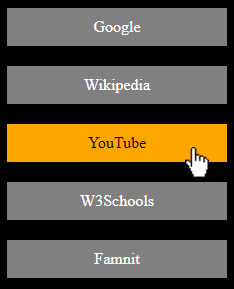
\includegraphics[width=5cm]{menu.png}
\end{figure}

\newpage

\section{JavaScript}

\noindent
Spodnja spletna stran prikazuje statičen napis ``\texttt{I Love FAMNIT!}''.

{\footnotesize
\begin{verbatim}
<!DOCTYPE html>
<html>
<head>
<title>Display</title>
</head>
<body>
<div id="display">I Love FAMNIT!</div>
</body>
</html>
\end{verbatim}
}

\noindent
Dodajte potrebno JavaScript kodo, da bo izpis animiran na sledeči način:
\begin{enumerate}
\item Na začetku je stran prazna.
\item Po 200 milisekundah se prikaže prva črka ``I''.
\item Po vsakih nadaljnjih 200 milisekundah se doda naslednji znak:
\begin{itemize}
\item ``I ''
\item ``I L''
\item ``I Lo''
\item \ldots
\item ``I Love FAMNIT!''
\end{itemize}
\item Celoten napis je prikazan 200 milisekund, nato pa se zbriše.
\item Postopek se ponavlja, dokler strani ne zapremo.
\end{enumerate}

\newpage

\section{PHP}

\noindent
Spodnja spletna stran izrisuje Hanojski stolp višine 6 ploščic. Ploščice so položene ena na drugo tako, da je manjša ploščica vedno na večji.

{\scriptsize
\begin{verbatim}
<!DOCTYPE html>
<html>
<head>
<title>Tower</title>
<style>
span {
    display: inline-block;
    height: 20px;
}
span.empty {
    background-color: white;
}
span.fill {
    background-color: blue;
}
</style>
</head>
<body>
<div>
<span class="empty" style="width:100px"></span><span class="fill" style="width:20px"></span>
</div>
<div>
<span class="empty" style="width:80px"></span><span class="fill" style="width:60px"></span>
</div>
<div>
<span class="empty" style="width:60px"></span><span class="fill" style="width:100px"></span>
</div>
<div>
<span class="empty" style="width:40px"></span><span class="fill" style="width:140px"></span>
</div>
<div>
<span class="empty" style="width:20px"></span><span class="fill" style="width:180px"></span>
</div>
<div>
<span class="empty" style="width:0px"></span><span class="fill" style="width:220px"></span>
</div>
</body>
</html>
\end{verbatim}
}

\noindent
Izpis kode HTML med značkama \texttt{<body>} in \texttt{</body>} generirajte s skripto PHP, tako da bo omogočala izrisovanje stolpa poljubne višine. Višina stolpa naj bo podana s povezavo do spletne strani, npr.: \texttt{http://\ldots/tower.php?height=10}. Če višina ni določena, naj se privzeto izriše stolp višine 6 ploščic.
\end{document}